\documentclass[11pt]{article}
\usepackage{amsfonts,amsmath,amssymb,amsthm,graphicx}
\usepackage{multirow}
\usepackage{booktabs}
\usepackage[caption=false]{subfig} 
\usepackage{color}
\usepackage{ifthen}
\usepackage[utf8]{inputenc}
\usepackage[english]{babel}
%\usepackage{physics}

\setlength{\topmargin}{0 mm}
\setlength{\oddsidemargin}{5 mm}
\setlength{\evensidemargin}{5 mm}
\setlength{\textwidth}{150 mm}
\setlength{\textheight}{210 mm}

\newtheorem{lemma}{Lemma}
\newtheorem{theorem}{Theorem}
\newtheorem{remark}{Remark}
\newcommand{\dzx}{D_0^x}
\newcommand{\dzxp}{D_{0p}^x}
\newcommand{\wdzx}{\widetilde{D_0^x}}
\newcommand{\wdzxp}{\widetilde{D_{0p}^x}}
\newcommand{\dpx}{D_+^x}
\newcommand{\dmx}{D_-^x}
\newcommand{\dzy}{D_0^y}
\newcommand{\dzyp}{D_{0p}^y}
\newcommand{\wdzy}{\widetilde{D_0^y}}
\newcommand{\dpy}{D_+^y}
\newcommand{\dmy}{D_-^y}
\newcommand{\dzz}{D_0^z}
\newcommand{\wdzz}{\widetilde{D_0^z}}
\newcommand{\dpz}{D_+^z}
\newcommand{\dmz}{D_-^z}
\newcommand{\dzt}{D_0^t}
\newcommand{\dpt}{D_+^t}
\newcommand{\dmt}{D_-^t}
\newcommand{\ehx}{E_{1/2}^x}
\newcommand{\ehy}{E_{1/2}^y}
\newcommand{\ehz}{E_{1/2}^z}
%
\newcommand{\calo}{{\cal O}}
%
\newcommand{\ab}{{\mathbf a}}
\newcommand{\bb}{{\mathbf b}}
\newcommand{\db}{{\mathbf d}}
\newcommand{\eb}{{\mathbf e}}
\newcommand{\fb}{{\mathbf f}}
\newcommand{\gb}{{\mathbf g}}
\newcommand{\ib}{{\mathbf i}}
\newcommand{\jb}{{\mathbf j}}
\newcommand{\nb}{{\mathbf n}}
\newcommand{\pb}{{\mathbf p}}
\newcommand{\tb}{{\mathbf t}}
\newcommand{\rb}{{\mathbf r}}
\newcommand{\yb}{{\mathbf y}}
\newcommand{\zb}{{\mathbf z}}
\newcommand{\qb}{{\mathbf q}}
\newcommand{\ub}{{\mathbf u}}
\newcommand{\vb}{{\mathbf v}}
\newcommand{\wb}{{\mathbf w}}

\newcommand{\Ab}{{\mathbf A}}
\newcommand{\Bb}{{\mathbf B}}
\newcommand{\Eb}{{\mathbf E}}
\newcommand{\Fb}{{\mathbf F}}
\newcommand{\Ib}{{\mathbf I}}
\newcommand{\Hb}{{\mathbf H}}
\newcommand{\Kb}{{\mathbf K}}
\newcommand{\Lb}{{\mathbf L}}
\newcommand{\Pb}{{\mathbf P}}
\newcommand{\Qb}{{\mathbf Q}}
\newcommand{\Rb}{{\mathbf R}}
\newcommand{\Ub}{{\mathbf U}}
\newcommand{\Tb}{{\mathbf T}}
\newcommand{\Xb}{{\mathbf X}}

\newcommand{\Abb}{\mathbb{A}}
\newcommand{\Bbbb}{\mathbb{B}}
\newcommand{\Ebb}{\mathbb{E}}
\newcommand{\Fbb}{\mathbb{F}}
\newcommand{\Ibb}{\mathbb{I}}
\newcommand{\Hbb}{\mathbb{H}}
\newcommand{\Kbb}{\mathbb{K}}
\newcommand{\Lbb}{\mathbb{L}}
\newcommand{\Pbb}{\mathbb{P}}
\newcommand{\Qbb}{\mathbb{Q}}
\newcommand{\Rbb}{\mathbb{R}}
\newcommand{\Ubb}{\mathbb{U}}
\newcommand{\Tbb}{\mathbb{T}}
\newcommand{\Xbb}{\mathbb{X}}
\newcommand{\Ybb}{\mathbb{Y}}
\newcommand{\Zbb}{\mathbb{Z}}

\newcommand{\uh}{\hat{u}}
\newcommand{\vh}{\hat{v}}
\newcommand{\ph}{\hat{p}}
\newcommand{\qh}{\hat{q}}

\newcommand{\re}{{\rm Re}\,}
\newcommand{\im}{{\rm Im}\,}

\renewcommand{\arraystretch}{1.3}
%
\newcommand{\p}{\partial}
%
\newcommand{\eq}{\!\!\! = \!\!\!}
\newcommand{\om}{\omega}
%\newcommand{\divergence}{\nabla\cdot}
%\newcommand{\curl}{\nabla\times}

\newcommand{\alphab}{\boldsymbol{\alpha}}
\newcommand{\lambdab}{\boldsymbol{\lambda}}
\newcommand{\psib}{\boldsymbol{\psi}}
\newcommand{\phib}{\boldsymbol{\phi}}
\newcommand{\Psib}{\boldsymbol{\Psi}}

\newcommand{\rhob}{\boldsymbol{\rho}}
\newcommand{\kab}{\boldsymbol{\kappa}}
\newcommand{\etab}{\boldsymbol{\eta}}
\newcommand{\zetab}{\boldsymbol{\zeta}}
\newcommand{\sigmab}{\boldsymbol{\sigma}}
\newcommand{\omegab}{\boldsymbol{\omega}}
\newcommand{\Gb}{{\mathbf G}}
\newcommand{\kb}{{\mathbf k}}
\newcommand{\sbold}{{\mathbf s}}
\newcommand{\ba}{\begin{array}}
\newcommand{\ea}{\end{array}}
\newcommand{\be}{\begin{equation}}
\newcommand{\ee}{\end{equation}}
\newcommand{\bd}{\begin{displaymath}}
\newcommand{\ed}{\end{displaymath}}
\newcommand{\pa}{\partial}
\newcommand{\f}{\frac}
\newcommand{\drp}{D^r_+}
\newcommand{\drm}{D^r_-}
\newcommand{\dqp}{D^q_+}
\newcommand{\dqm}{D^q_-}
\newcommand{\dtqn}{\widetilde{{D^q_0}} }
\newcommand{\dtrn}{\widetilde{{D^r_0}} }
\newcommand{\dqn}{D^q_0}
\newcommand{\drn}{D^r_0}
\newcommand{\erh}{E^r_{1/2}}
\newcommand{\eqh}{E^q_{1/2}}

\def\dpl{D_+}
\def\dmi{D_-}

\newcommand{\ubbar}{\bar{\mathbf{u}}}
\newcommand{\ubar}{\bar{u}}

% Numerical solutions
% \newcommand{\vb}{\mathbf{v}}


% Grids
\newcommand{\xb}{\mathbf{x}}
\newcommand{\ybh}{\hat{\mathbf{x}}}
\newcommand{\xbh}{\hat{\mathbf{x}}}
\newcommand{\Ja}{J_{\alpha}}
\newcommand{\ga}{g_{\alpha}}
\newcommand{\Ma}{M_{\alpha}}

% Interpolation
\newcommand{\Nxy}{N_{\mathbf{x}\rightarrow\hat{\mathbf{x}}}}
\newcommand{\Nyx}{N_{\hat{\mathbf{x}}\rightarrow\mathbf{x}}}
\newcommand{\Nuv}{N_{\bar{\ub}_1\rightarrow\bar{\ub}_2}}
\newcommand{\Nvu}{N_{\bar{\ub}_2\rightarrow\bar{\ub}_1}}
\newcommand{\Nij}{N_{\bar{\ub}_i\rightarrow\bar{\ub}_j}}
\newcommand{\Nji}{N_{\bar{\ub}_j\rightarrow\bar{\ub}_i}}
\newcommand{\Px}{P}
\newcommand{\Pxh}{\hat{P}}

% Domains
\newcommand{\domp}{\Omega_{p}}
\newcommand{\domu}{\Omega_{\ub}}
\newcommand{\domv}{\Omega_{\vb}}
\newcommand{\domui}{\Omega_{\bar{\mathbf{u}}_i}}
\newcommand{\domuj}{\Omega_{\bar{\mathbf{u}}_j}}
\newcommand{\gamja}{\Gamma_{j0}}
\newcommand{\gamjb}{\Gamma_{j1}}
\newcommand{\gamia}{\Gamma_{i0}}
\newcommand{\gamib}{\Gamma_{i1}}

% Comments
\newcommand{\red}{\color{red} AP:}
\newcommand{\usecomments}{true}
\newcommand{\ocomment}[1] {
\ifthenelse{ \equal{\usecomments}{true} }{
 \textbf{Ossian: }{\color{blue} #1}
}{
}
}



\begin{document}

\title{Final Report Internship - Quantum Control}
\author{Ylva Rydin}

% TODO: Design a nice front page here

\date{\today}

\maketitle
\section{Introduction}

We want to design a gate that transforms a quantum state $\psi_0$ to a target state $d$. 
A simple example of such a gate is the SWAP-gate that swaps the quantum state  
%
\[
\psi_s =  a_0 |00\rangle + a_1 |01\rangle + a_2 |10\rangle + a_3 |11 \rangle, 
\]
%
into
%
\[
d_s =  a_0 |00\rangle + a_2 |01\rangle + a_1 |10\rangle + a_3 |11 \rangle. 
\]
%
Quantum gates can be seen as unitary operations $d = U_g \psi_0.$ For example, the SWAP gate above is represented by the matrix:
%
\begin{equation} \label{eq:SWAPgate}
U_s =
\begin{bmatrix}
1 & 0 & 0 & 0 \\
0 & 0 & 1 & 0 \\
0 & 1 & 0 & 0 \\
0 & 0 & 0 & 1
\end{bmatrix}.
\end{equation}

In the quantum computer, the time evolution of the quantum states is governed by the time-dependent Schr\"odinger equation,

\begin{equation}\label{eq:schrodinger_example}
\frac{d \psib(t)}{dt} + iH(t)\psib(t)=0,\quad 0\leq t\leq T, \quad \psib (0) = \psi_0.
\end{equation}

The goal in this project is to determine a control function for the quantum computer that realizes a Hamiltonian $H(t)$ such that the final time solution to \eqref{eq:schrodinger_example} is $\psi(T) = d$. It is possible to show that for each unitary gate, there exist a control function that realizes this for some $T < \inf $ whch is shown in chapter 4 in Borzì et al. \cite{Borzi-17}. One realization of the SWAP-gate \eqref{eq:SWAPgate}  computed with the methods described in this report in shown in Figure \ref{fig:responseSWAP}. In this figure, the response is shown for the four initial conditions $\psi(0) = \mathbf{e}_j$ , $j = 1,2,3, 4$. Here $\mathbf{e}_j$ is the $j^{th}$ canonical unit vector (zero, except element $j$ which is one). In this example $T = 150 ns$, for this SWAP-gate the time-dependent Hamiltonian is

\begin{equation}
H(t)= H_0 + p(t)H_c, 
\end{equation}

where

\[
H_0 = 
\begin{bmatrix}
0 & 0 & 0 & 0 \\
0 & \omega_2 & 1 & 0 \\
0 & 0 & \omega_3 & 0 \\
0 & 0 & 0 & \omega_4
\end{bmatrix},
\quad
H_c =
\begin{bmatrix}
0 & 1 & 0 & 0 \\
1 & 0 & 0 \sqrt{2} & 0 \\
0 & \sqrt{3} & 0 & \sqrt{3} \\
0 & 0 & \sqrt{3} & 0
\end{bmatrix}.
\]
where {\color{red} $\omega_i$ are the frequencies of the states in the experimental}. The control signal $p(t)$ is shown in Figure \ref{fig:controlfunc}. Main goal of this project is to develop a mathematical framework and implement a code that can compute control functions for different quantum gates.
{\color{red} 
The difficult parts are ....

The focus of the internship has been to ...

The remainder of this report ...}


\begin{figure}
  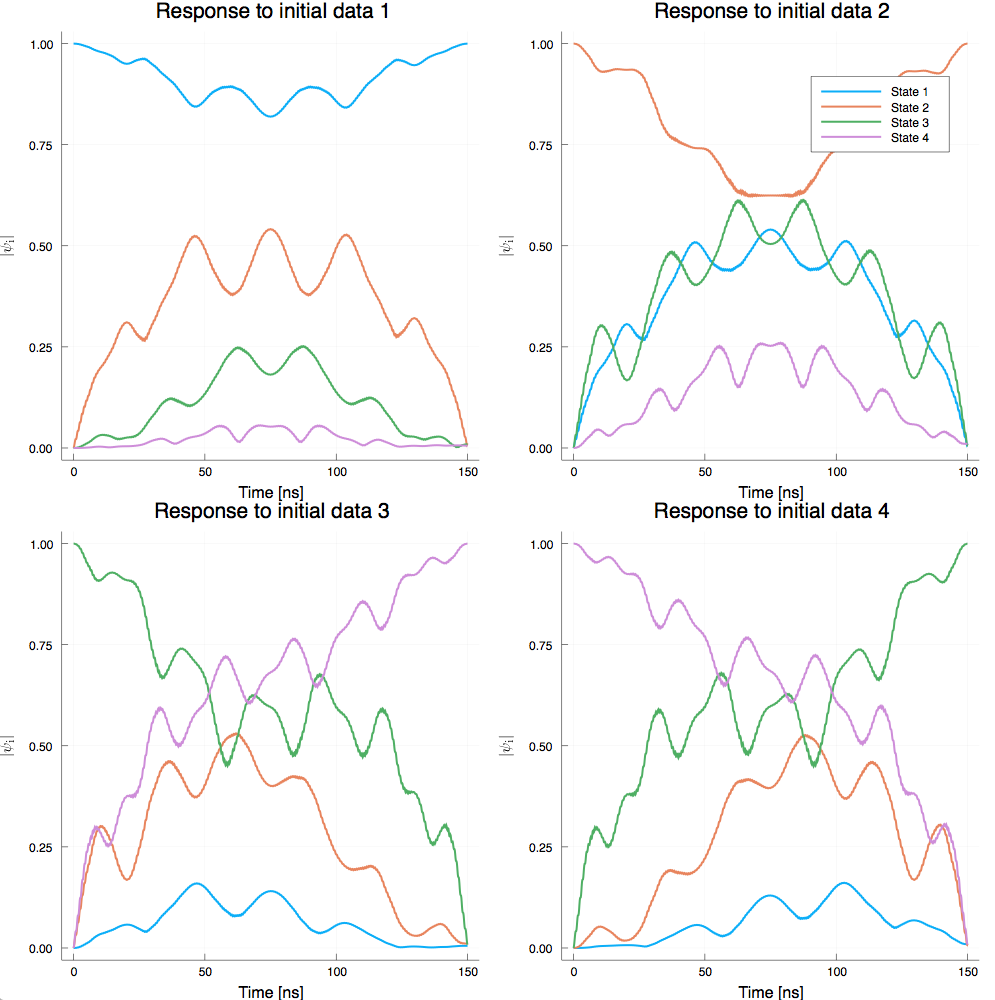
\includegraphics[width=\linewidth]{response}
  \caption{Response from the SWAP-gate}
  \label{fig:responseSWAP}
\end{figure}

\begin{figure}
  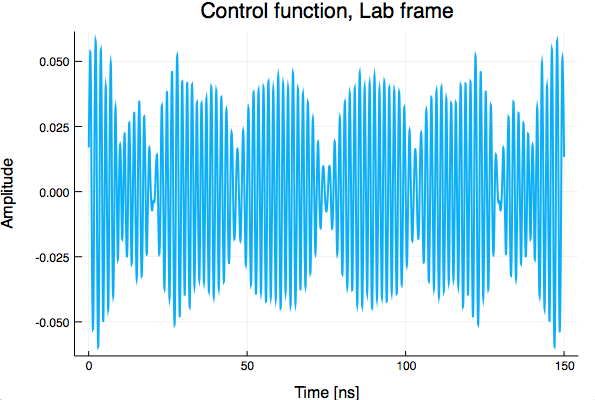
\includegraphics[width=\linewidth]{controlfunc}
  \caption{Control function for the SWAP-gate}
  \label{fig:controlfunc}
\end{figure}

\begin{itemize}
  \item Background, why do we need to do this 
  \item More background: What is done and why is this not good enough
  \item Background Adjoint
  \item Something about Julia
  \item An overview of the full report, what is the main purpouse o the project
\end{itemize}

%
%
%
%
\section{The Control Problem} \
In this section, an objective functional for optimizing a general gate $d = U_g \psi_0$ is derived. Subsecection \ref{subsec:Adjoint}  functional that measures the infidelity of the final state is presented. Further, it is shown how to compute it's gradient by solving the adjoint state equation. In the subsections \ref{subsec:guarlevels} and \ref{subsec:penalty} additions to the functional required to ensure that the control signal is feasible to run on the physical machine are presented.

\subsection{The adjoint method} \label{subsec:Adjoint}
Let the wave functions $\psib_j(t,\alphab)\in [0, T]\times \mathbb{R}^D \to \mathbb C^N$ be governed by the Schr\"odinger equation,
\begin{equation}\label{eq:schrodinger}
\frac{d \psib_j}{dt} + iH(t,\alphab)\psib_j=0,\quad 0\leq t\leq T, \quad \psib_j(0)=\eb_j,\quad j=1,2,\ldots,N.
\end{equation}
The Hamiltonian matrix satisfies
\[
H(t,\alphab) = H_0 + p(t,\alphab)H_c,\quad H(t,\alphab) = H^\dag(t,\alphab),
\]
where $p(t,\alphab)$ is a scalar function of time that depends on the parameter vector
$\alphab=[\alpha_1,\alpha_2,\ldots,\alpha_D]^T\in \mathbb R^D$. We introduce
\[
\phib_{jk}(t,\alphab) = \frac{\p \psib_j (t,\alphab)}{\p \alpha_k},\quad k=1,2,\ldots,D.
\]
By differentiating \eqref{eq:schrodinger} with respect to $\alpha_k$,
\begin{align}
\frac{d \phib_{jk}}{dt} + iH(t,\alphab)\phib_{jk}&=\fb_{jk}(t,\alphab),\quad 0\leq t\leq T, \quad
\phib_{jk}(0)=0,\label{eq_pert_schrodinger}\\
%
\fb_{jk}(t,\alphab) &= -i \frac{\p p(t,\alphab)}{\p \alpha_k} H_c \psib_j(t,\alphab).\label{eq_pert_force}
\end{align}
%
Let $U_g = [\db_1, \db_2, \ldots, \db_N]\in \mathbb{C}^{N\times N}$, represent the target unitary
gate ($U_g^{-1} = U_g^\dag$) and collect the wave functions for the different initial data in the
unitary matrix $U = U(T,\alpha) \in \mathbb C^{N\times N}$, where
%
\begin{equation}\label{eq:udef}
U = \left[ \psib_1, \psib_2, \ldots, \psib_N \right],\quad U^\dag = U^{-1}.
\end{equation}
%
An objective functional that measures the infidelity in the final unitary is given by
%
\begin{equation}\label{eq:objf}
g_1(U(T,\alphab)) = 1 - \frac{1}{N^2} \left| S_T(\alphab) \right|^2,\quad S_T(\alphab) = \left\langle U(T,\alphab), U_g \right\rangle_F.
%
\end{equation}
The Fr\"obenius matrix scalar product between square complex-valued matrices $A$ and $B$ is defined by
\begin{equation}\label{eq:frobenius}
\left\langle A, B\right\rangle_F = \mbox{tr$\left( A^\dag B\right)$} = \sum_{j=1}^N \langle \ab_j, \bb_j\rangle_2,
\end{equation}
%
where $A=[\ab_1, \ab_2, \ldots, \ab_N]$ and  $B=[\bb_1, \bb_2, \ldots, \bb_N]$. Differentiating
%
\eqref{eq:objf} with respect to $\alpha_k$ gives the gradient,
\begin{equation}\label{eq:objgrad}
\frac{\p g_1}{\p \alpha_k} = - \frac{2}{N^2} {\rm Re}\! \left(\frac{\p S_T}{\p \alpha_k} \overline{S}_T \right).
\end{equation}

In this work we compute the gradient by solving the adjoint equation,
\begin{equation}\label{eq:adjoint}
-\dot{\lambdab}_j - iH(t,\alphab)\lambdab_j=\boldsymbol{\gamma}_j(t),\quad T\geq t\geq 0, \quad \lambdab_j(T)=\qb_j,\quad j=1,2,\ldots,N.
\end{equation}
%
Note that this equaton is closeley related to \ref{eq:schrodinger}. This equation is solved backwards in time and is subject to a termianl condition.

\begin{theorem}
If the forcing function $\boldsymbol{\gamma}_j(t) = 0$, and the terminal condition $\qb_j = -\overline{S}_T \db_j/N^2$ then

\begin{equation}\label{eq:sensitivity}
  \frac{\p g_1}{\p \alpha_k} = 
  2 {\rm Re}\! \sum_{j=1}^N \int_0^T \langle \fb_{jk},\lambdab_j \rangle_2\, d\tau.
\end{equation}
\end{theorem}

\begin{proof}
Consider
\begin{multline}
  I:= \int_0^T \langle \phib_{jk}, \boldsymbol{\gamma}_j \rangle_2\, d\tau =  \int_0^T \langle \phib_{jk},
  -\dot{\lambdab}_j - iH(t,\alphab)\lambdab_j \rangle_2\, d\tau \\
  %
  =  -\int_0^T \langle  \phib_{jk},
  \dot{\lambdab}_{j} \rangle_2\, d\tau +  \int_0^T \langle iH(t,\alphab) \phib_{jk},\lambdab_j \rangle_2\, d\tau.
\end{multline}
By integration by parts,
\begin{multline*}
\int_0^T \langle  \phib_{jk}, \dot{\lambdab}_{j} \rangle_2\, d\tau =
%
\left[ \langle \phib_{jk}, \lambdab_j \rangle_2 \right]_0^T - \int_0^T \langle  \dot{\phib}_{jk},
\lambdab_{j} \rangle_2\, d\tau\\
%
= \langle \phib_{jk}(T), \qb_j \rangle_2  - \int_0^T \langle  \dot{\phib}_{jk}, \lambdab_{j} \rangle_2\, d\tau,
\end{multline*}
because $\phib_{jk}(0)=0$ and $\lambdab_j(T) = \qb_j$. Thus,
\begin{multline*}
I = -\langle \phib_{jk}(T), \qb_j \rangle_2 + \int_0^T \langle \dot{\phib}_{jk} + iH(t,\alphab)
\phib_{jk},\lambdab_j \rangle_2\, d\tau\\
%
= -\langle \phib_{jk}(T), \qb_j \rangle_2 + \int_0^T \langle \fb_{jk},\lambdab_j \rangle_2\, d\tau.
\end{multline*}
Therefore,
\begin{equation}\label{eq:adjointrel}
 \langle \phib_{jk}(T), \qb_j \rangle_2 + \int_0^T \langle \psib_{jk},\boldsymbol{\gamma}_j\rangle_2\, d\tau = \int_0^T \langle \fb_{jk},\lambdab_j \rangle_2\, d\tau.
\end{equation}
where $\fb_{jk}(t)$ is given by \eqref{eq:pertforce}. Choosing $\qb_j = -\overline{S}_T \db_j/N^2$ and $\boldsymbol{\gamma}_j(t)=0$ gives
\begin{equation}\label{eq:sensitivity}
  \frac{\p g_1}{\p \alpha_k} =  2 {\rm Re}\! \sum_{j=1}^N \left\langle \phib_{jk}(T,\alphab),
  \qb_j\right\rangle_2 =
  %
  2 {\rm Re}\! \sum_{j=1}^N \int_0^T \langle \fb_{jk},\lambdab_j \rangle_2\, d\tau.
\end{equation}
\end{proof}



\subsection{Discouraging Population of Higher Energy States} \label{subsec:guarlevels}
The quantum computer is a sensitive system and its design imposes additional constraints on the control function. 
Firstly, since the actual Hamiltonian system is in general infinite-dimensional we need to ensure that our gate does not polulate higher energy states. Therefore, an additional term in the objective functional is added to supress highly energetic states. How many such "guard terms" that are required depends on the target gate. 

Let $N_g\geq 0$ denote the number of guard states and expand the wave
function such that $\psib_j(t,\alphab)\in [0, T]\times \mathbb{R}^D \to \mathbb{C}^{N_t}$, where
$N_{t} = N + N_g$. The Schr\"odinger equation \eqref{eq:schrodinger} still governs the evolution of
$\psib_j(t,\alphab)$, but now also models the evolution of the guard states. As a result the
Hamiltonian matrix $H(t)$, but is now of size $N_t\times N_t$. The forcing function $\fb_{jk}(t,\alphab)$
is now a vector with $N_t$ elements. The matrices $U(t,\alphab)$ and $U_g$ are now represented by
rectangular matrices with $N_t$ rows and $N$
columns,
\[
U = [ \psib_1, \psib_2, \ldots, \psib_N ],\quad 
U_g = \begin{bmatrix}
\db_1 & \db_2 & \ldots & \db_N \\
\boldsymbol{0} & \boldsymbol{0} & \ldots & \boldsymbol{0}
  \end{bmatrix}.
\]
Here, the zero vector $\boldsymbol{0} \in \mathbb{R}^{N_g}$. Thus, the definition of the objective
function $g_1$ in \eqref{eq:objf} still holds. Furthermore, only the first $N$ elements of $\psib_j$
and $\phib_{jk}$ matter because the last $N_g$ rows of $U_g$ are identically zero. To accomodate for
the guard levels, the terminal condition for the adjoint wave equation \eqref{eq:adjoint} becomes
\begin{equation}\label{eq:adjointtc}
\lambdab_j(T) = -\frac{\overline{S}_T}{N^2} \begin{bmatrix}
  \db_j \\
  \boldsymbol{0}
  \end{bmatrix}.
\end{equation}
%
To measure the population of the guard levels we define the functional
\begin{equation}\label{eq:g2}
  g_2(U(\alphab)) =\int_0^T \sum_{j=1}^N \left\langle \psib_j(\tau,\alphab), W\psib_j(\tau,\alphab)
  \right\rangle_2\, d\tau,
\end{equation}
where $W$ is a real diagonal matrix with zero entries in the first $N$ rows and columns,
\[
W = \begin{bmatrix}
  0 &&&&& \\
  & \ddots &&&& \\
  && 0 &&& \\
  &&& w_1 && \\
  &&&& \ddots & \\
  &&&&& w_{N_g}
\end{bmatrix},\quad 0 < w_1 \leq w_2 \leq \ldots \leq w_{N_g}.
\]
The gradient of $g_2$ satisfies
\[
\frac{\partial g_2}{\partial \alpha_k} = 2\,{\rm Re}\! \sum_{j=1}^N  \int_0^T \left\langle \phib_{jk}(\tau,\alphab), W\psib_j(\tau,\alphab)
\right\rangle_2\, d\tau.
\]
The gradient of the combined objective functional
\[
g(\alphab) = g_1(\alphab) + g_2(\alphab),
\]
therefore satisfies
\[
\frac{\partial g}{\partial \alpha_k} = 2 {\rm Re}\! \sum_{j=1}^N \left(
%
-\left\langle\phib_{jk}(T,\alphab), \frac{\overline{S}_T}{N^2} \db_j \right\rangle_2 +
%
\int_0^T \left\langle \phib_{jk}(\tau,\alphab), W\psib_j(\tau,\alphab)\right\rangle_2\, d\tau \right).
\]
Note that each term in the sum is of the type \eqref{eq:sensitivity}. Thus, we can compute the
gradient using the previous approach by solving the adjoint equation \eqref{eq:adjoint} with
terminal condition \eqref{eq:adjointtc} and forcing function $\boldsymbol{\gamma}_j = W \psib_j$.

   
\subsection{Penalty for high amplitudes}\label{subsec:penalty}

The experimantal rif has a limit on the amplitude of the conrol-signal $\alpha_{max} > 0$. To penalize amplitudes close to or above this limit the term
%
\begin{equation}\label{eq:g3}
g_3(\alpha) = -2\log(2) - \frac{1}{k}\sum_{k=1}^m \log((\alpha_{max}^2-\alpha_k^2)/(2\alpha_{max})^2),
\end{equation}
%
is added to the functional. Here $\log$ denotes the natural logarithm. This additional term has the gradient

\begin{equation}\label{eq:g3grad}
\frac{\partial g_3}{\partial \alpha_k} = -\frac{1}{k} \frac{2\alpha_k}{\alpha_{max}^2-\alpha_k^2}.
\end{equation}
The complete objective functionnal is obtained by adding a weighted sum of \eqref{eq:objf}, \eqref{eq:g2}, and \eqref{eq:g3},
%
\begin{equation}
g(\alpha) = s_1 g_1(\alpha) + s_2 g_2(\alpha) + s_3 g_3(\alpha) 
\end{equation}
%
where $s_1,  \ s_2, \ s_3 \geq 0 $ are scale factors  for the different components.

\section{Implementation}

There exists a prototype implementation of an earlier version this control problem has been implemented in Octave \cite{octave}. 
However, this implementation is slow already on small problem sizes. 
Hence, there was need for a new implementation in order to solve larger and more complex control problems in the future. 
In this project, a solver for the control-problem has been implemented in Julia \cite{juliaDoc}. Julia is a dynamic language that is designed to be as easy to use as for example MATLAB, Octave or Python while having a performance as traditional high-performance languages such as  C \cite{} or FORTRAN \cite{fortran}. 


The goal is that the Julia-implementation of the control-problem should be simple enough to allow fast prototyping while the project develops while still being fast and scalable enough to solve large-scale problems in the future. Our hope is that this is a more efficient workflow that prototyping on Octave or MATLAB and then translating the code to a high-performance language. In the future we aim to solve larger control problems that will require parallelization.  For parallel computing, both by a native parallelization package and by interfaces to parallelization libraries such as CUDA \cite{CUDA} and MPI \cite{MPI}.

The Julia-implementation is still in a prototype stage and has not yet been parallelized, but already the optimization has shown to be about 100 times faster than the Octave code. The Julia-code consist of three modules. The first module "bsplines.jl" represents the control function in a basis of quadratic polynomials. The second module, "objfunc.jl" computes the objective functional \ref{eq:totobjective} and its gradient. The third module "timestep.jl" integrates the control problem with a Str\"omer-Verlet time integration. For optimization, the (L)-BFGS algorithm in Julia package "Optim.jl" is used. In the remainder of this section, some important details about the numerical methods implement in these modules are described.


\subsection{Representing the Control Function by Qubic B-splines}
In the control problem, the control function $p(t,\alpha) \in [0, T]$ is represented by a basis of quadratic polynomials as
%
\begin{equation}\label{eq:control_splines}
p(t,\alpha) = \sum_{k = 1}^D \alpha_k B_k(\tau(k,t)), 
\end{equation}
%
where $D$ is the number of splines, the scaled time parameter $\tau(k,t) = \frac{t- h_{k}(k-1.5)}{3h_{k}}$ and $h_{k} = T/(D-2)$. The the basis functions are

\begin{align}\label{eq:splinebasis}
B_k(\tau(k,t)) = 
\begin{cases} 
0, \quad &t < (k - 3)h_k, \\
9/8 + 4.5 \tau(k,t) + 4.4 \tau(k,t)^2, \quad &(k - 3)h_k \leq t < (k - 2)h_k, \\
0.75 - 9 \tau(k,t)^2, \quad  &(k-2)h_k \leq t <  (k-1)h_k, \\
9/8 + 4.5 \tau(k,t) + 4.4 \tau(k,t)^2, \quad &(k-1)h_k \leq t < kh_k,\\
0, \quad &kh_k\leq t. 
\end{cases}
\end{align}

\subsection{Computing the Objective Functional and its Gradient}
In the implementation we cosider solutions to the Schr\"odinger equation \ref{eq:schrodinger} on the form
%
\[
H(t) = H_0 = p(t,\alpha)(a + a^\dagger)
\]
%
Where the costant partof the hamiltonian is the diagonal matrix 
\[
H_0 = 
\begin{bmatrix}
0 & & & & \\
& \omega_2 & & & \\
& & \omega_3 & & \\
& & & \ddots & \\
& & & & \omega_N \\
\end{bmatrix}
\]
%
and
%
\begin{equation*}\label{eq_matrices}
%
a = \begin{bmatrix}
0 & 1 & & & & &\\
 & 0 & \sqrt{2} & & & &\\
&  & 0 & \sqrt{3} & & &\\
& &  & \ddots & \ddots & &\\
& & & &  0 & \sqrt{N} & \\
& & & & & 0&
\end{bmatrix},\quad
%
a^\dag = \begin{bmatrix}
0 &  & &  &\\
1 & 0 & & & &\\
&  \sqrt{2} & 0 &  & &\\
& &  \sqrt{3} & 0 & &\\
& &  & \ddots & \ddots & \\
& & & & \sqrt{N} & 0
\end{bmatrix}
\end{equation*}
%
and $p(t,\alpha)$ is a real valued control function. In the code, a transformed version of \eqref{eq:schrodinger} that is less stiff and hence allows equation to be solved with a larger time step. In the code, the rotaded system

\begin{equation}\label{eq:rotschroedinger}
\frac{d\tilde{\psi}}{dt} = - i \tilde{H}(t)\tilde{\psi}, \quad \tilde{H}(t) =  p(t,\alpha)(R(t)aR^\dag(t) + R(t)a^\dag R^\dag(t))
\end{equation}
is solved where the rotation matrix
\\
\[
R = 
\begin{bmatrix}
 1 & & & & \\ 
 & e^{i \omega_1 t} & & &\\
 & & e^{i \omega_2 t} & &\\
 & & &\ddots &  \\
 & & & & e^{i \omega_N t}
\end{bmatrix}
\]
is solved according to the methodology discribed in \ref{sec:Adjoint}.

In the code, the rotated Schr\"odinger equation \eqref{eq:rotschroedinger} is first solved and the gradient is computed with the trapetsoidal rule. Then the Adjoint equation and the forward problem are solved together backwards. By doing this, the solution from the forward problem does not have to be stored to compute the backwards problem which will be beneficial when the problem size is increased. When solving the backward problem, the gradient is numerically computed with trapetsiodal rule.

\subsection{Time integration}
To utilize efficient numerical ODE solvers it is desirable to derive a real-valued equivalent of \label{eq:rotschroedinger}.
Let the real-valued functions $v_r$ and $v_i$ be defined by
%
\begin{equation}
\tilde{\psi} = v_r + i v_i 
\end{equation}
%
and decompise the hamiltionian into $\tilde{H}(t) = K(t) + iS(t)$, where $K$ is real-valued and symmetric and $S$ is real valued and skew-symmetric.
Thus, we have
%
\begin{align}
&\tilde{H}\tilde{\psi} = (K + iS)(u + iv) = (Ku + Sv) + i(Su - Kv), \\
&-i\tilde{H} = -i(Ku + Sv) + (Su -Kv).
\end{align}
%
Therfore, a real valued equivalent of  \eqref{eq:rotschroedinger} is
%
\begin{equation}\label{eq:realshrodinger}
  \begin{bmatrix} \dot{u}\\ \dot{v} \end{bmatrix} =
%
  \begin{bmatrix}
    S(t) & -K(t) \\ K(t) & S(t)
  \end{bmatrix}     
  %
  \begin{bmatrix} u\\ v \end{bmatrix} .
\end{equation}

To solve \eqref{eq:realschroedinger} numerically, we discretize time on a grid with $t_n = n
\delta_t$, $n=0,1,2,,\ldots$. Here, the time step ($\delta_t$) is constant, but this assumption can
be relaxed. We denote the numerical solution $u^n\approx u(t_n)$ and $v^n\approx v(t_n)$.  In
general, $S(t)\ne0$ and the Hamiltonian system is non-separable. Givent $(u^n, v^n)$, the 
Str\"omer-Verlet scheme evolves the solution by
\begin{align*}
  \left(I - \frac{\delta_t}{2} S^{n}\right) \ell_1 &= K^n u^n + S^n v^n + F_v^n,\\
%
  v^{n+1/2} &= v^n + \frac{\delta_t}{2}\ell_1,\\
  %
  \kappa_1 &= S^{n+1/2} u^n - K^{n+1/2} v^{n+1/2} +
  F_u^{n+1/2},\\
%
  \left(I - \frac{\delta_t}{2} S^{n+1/2}\right) \kappa_2 &= S^{n+1/2}\left( u^n + \frac{\delta_t}{2}
  \kappa_1 \right) - K^{n+1/2}  v^{n+1/2} + F_u^{n+1/2},\\
  %
  u^{n+1} &= u^n + \frac{\delta_t}{2}\left( \kappa_1 + \kappa_2 \right),\\
%
  \ell_2 &= K^{n+1} u^{n+1} + S^{n+1}  v^{n+1/2} + F_v^{n+1},\\
  %
  v^{n+1} &= v^n + \frac{\delta_t}{2}\left( \ell_1 + \ell_2 \right).
\end{align*}
%
The above Str\"omer-Verlet scheme is second order accurate, symplectic and time reversible. By using a
compositional technique where each time-step is decomposed into several sub-steps, the order of
accuracy can be raised. Fourth order accuracy can be obtained with three sub-steps, sixth order with
seven or nine sub-steps, and eight order requires at least fifteen sub-steps, see Harirer et
al.~\cite{HairerLubichWanner-06} for further details.

\subsection{Verification}
finite diff, forward component of gradient,


\section{Numerical Results}

\begin{itemize}
  \item Show results (different gates and control functions) and so on
\end{itemize}
\section{Experimental Results}
If there are any successfull ones

\section{Discussion and future development}
\begin{itemize}
  \item Verification qtip
  \item implement an other time integrator or solve the non rotated system to make sure that rotations does not skrew up anything
  \item Faster code
  \item Paralell code
  \item Dual consistency
  \item verify by existing python code
  \item run sucessful experiments
  \item change objective func? 
\end{itemize}

\bibliographystyle{plain}
\bibliography{quantum}
\end{document}
